%pseudo code here defined with macro because else tabs won't reamin

\section{Introduction}

\begin{frame}
	\frametitle{What is a PID controller?}
	\small{
	\begin{definition}
		A \textbf{P}roportional-\textbf{I}ntegral-\textbf{D}eriviative (PID) controller is a control-loop feedback mechanism (controller) widely used in process industry.
		\begin{figure}
			\centering
			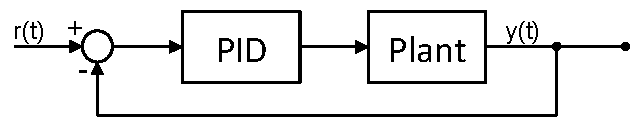
\includegraphics[width=0.8\linewidth]{PID_figure}
		\end{figure}
		\vspace{-1em}
		Continuous-time text book equation:
		\begin{equation*}
			u(t) = 	\underbrace{\vphantom{\int^t_0e(\tau)d\tau}K_p e(t)}_\text{Proportional Action} 
					+ \underbrace{K_i\int^t_0e(\tau)d\tau}_\text{Integral Action} 
					+ \underbrace{\vphantom{\int^t_0e(\tau)d\tau} K_d \frac{de(t)}{dt}}_\text{Derivative Action}
		\end{equation*}
		\vspace{-1.5em}
	\end{definition}
	
	\textbf{Note:} $90$\% (or more) of control-loops in process industry are PID.\\ 
}
\end{frame}

\begin{frame}
	\frametitle{What is a PID controller?}
	\footnotesize{
	\begin{itemize}
		\item \textbf{P}roportional action $u_p(t) = K_p e(t)$: it depends on the instaneous value of the error. 
			\begin{itemize}
				\pro Reduces rise time
				\pro Reduces but \textbf{does not eliminate the steady-state error}: Only when $K \rightarrow \infty , \text{error} \rightarrow 0$
				 (unless the plant has pole(s) at $s=0$)
			\end{itemize}
		\item \textbf{I}ntegral action $u_i(t) =K_i\int_0^t e(\tau)d\tau$: it is proportional to the accumulated error.
			\begin{itemize}
				\pro \textbf{Eliminates the steady-state error} for a constant or step input (e.g., in plants of type 0)
				\con Makes transient response slower 
			\end{itemize}
	
		\item \textbf{D}erivative action $u_d(t) = K_d \frac{de(t)}{dt}$: it is proportional to the rate of change of the error. 
			\begin{itemize}
				\pro Increases the stability of the system, reduces overshoot, improves the transient response
				\con Amplifies the noise present in the error signal
			\end{itemize}
	\end{itemize}}
\end{frame}

\section{Analog and Digital formulations}

\begin{frame}
	\frametitle{Proportional Control}
	The continuous-time and discrete-time implementations are identical.\\
	\vspace{1em}
	For the continuous-time case we have:
	\begin{equation*}
		u_p(t) = K_p e(t) \quad \rightarrow \quad \frac{U_p(s)}{E(s)} = K_p 
	\end{equation*}
	and for the discrete-time case:
	\begin{equation*}
		u_p[k] = K_p e[k] \quad \rightarrow \quad \frac{U_p(z)}{E(z)} = K_p 
	\end{equation*}µ
	where e(t) or e[k] is the error signal.
\end{frame}

\begin{frame}
	\frametitle{Derivative Control}
	In continuous-time it is given by:
	\begin{equation*}
		u_d(t) = K_d \frac{de(t)}{dt} \quad \rightarrow \quad \frac{U_d(s)}{E(s)} = K_d s 
	\end{equation*}
	and in discrete-time by (using backward Euler):
	\begin{equation*}
	u_d[k] = K_d \frac{ e[k] - e[k-1]}{T_s} \quad \rightarrow \quad \frac{U_d(z)}{E(z)} = K_d \frac{z - 1}{T_sz}
	\end{equation*}
	with $T_s$ the sampling time.
\end{frame}

\begin{frame}
	\frametitle{Integral Control}
	In continuous-time it is given by:
	\begin{equation*}
		u_i(t) = K_i \int_0^t e(\tau)d\tau \quad \rightarrow \quad \dot{u_i}(t) = K_i e(t) \quad \rightarrow \quad \frac{U_i(s)}{E(s)} = \frac{K_i}{s} 
	\end{equation*}
	and in discrete-time by (using backward Euler)
	\begin{equation*}
	u_i[k] = u_i[k-1] + K_i T_s e[k] \quad \rightarrow \quad \frac{U_i(z)}{E(z)} = K_i \frac{z T_s}{z - 1}
	\end{equation*}
	with $T_s$ the sampling time.
\end{frame}

\begin{frame}
	\frametitle{Digital formulation (conventional version)}
	\vspace{-1em}
	\small{
	\begin{block}{Digital PID controller (conventional version)}
			\vspace{-1em}
			%Difference equations
			\begin{align*}
			u[k] &= K_p e[k] + \frac{K_d}{T_s}(e[k] - e[k-1])+u_i[k] \\
			&\text{with } u_i[k] = u_i[k-1] + K_i T_s e[k]
			\end{align*}	
			In the $\mathcal{Z}$-domain:
			\begin{equation*}
			\frac{U(z)}{E(z)} = \textcolor{red}{K_p}  + \textcolor{red}{K_i T_s}\frac{z}{z-1} + \textcolor{red}{\frac{K_d}{T_s}}\frac{z-1}{z}
			\end{equation*}
			where $K_iT_s$ and $\frac{K_d}{T_s}$ are the new derivative and gains.
	\end{block}
	\begin{columns}
		\begin{column}{0.5 \textwidth}
			\begin{block}{Digital PI controller}
				$$\frac{U(z)}{E(z)} = K_p + K_i T_s \frac{z}{z-1} $$
			\end{block}
		\end{column}
		\begin{column}{0.5 \textwidth}
			\begin{block}{Digital PD controller}
				$$\frac{U(z)}{E(z)} = K_p + \frac{K_d}{T_s}\frac{z-1}{z} $$
			\end{block}
		\end{column}
	\end{columns}}
	%\vspace{1em}
\end{frame}

\begin{frame}
	\frametitle{Alternative Digital PID controller}
	If we discretize the continuous-time (analog) PID controller using the bilinear transformation,
	\begin{align*}
	\frac{U(z)}{E(z)} &= \left. K_p + \frac{K_i}{s} + K_d s \right|_ {s=\frac{2}{T_s}\left( \frac{z-1}{z+1}\right)}
	\end{align*}
	we obtain an alternative form for a digital PID controller
	\begin{align*}
		\frac{U(z)}{E(z)} &= K_p + \frac{K_iT_s(z + 1)}{2(z-1)} + \frac{2K_d(z-1)}{T_s(z+1)} \\
		&= \frac{\alpha_2 z^2 + \alpha_1 z + \alpha_0}{(z-1)(z+1)}
	\end{align*}
	where $\alpha_2, \alpha_1, \alpha_0$ are design parameters.
\end{frame}

\begin{frame}
	\frametitle{PID Math Demystified}
	\begin{figure}
\centering
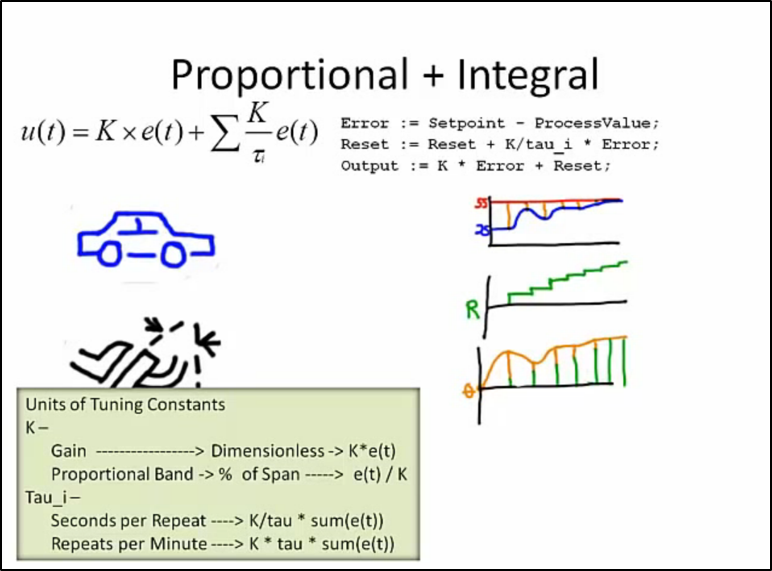
\includegraphics[width=0.7\linewidth]{img/PID_video}
\end{figure}
	\url{https://www.youtube.com/watch?v=JEpWlTl95Tw}
\end{frame}

\begin{frame}
	\frametitle{Alternative Derivative Action (Continuous-time)}
		\begin{columns}
			\begin{column}{0.7\linewidth}
				Imagine a step change in reference signal $r(t)$. 
				This results in a theoretically infinite, practically very large response of
				the derivative term.  
			\end{column}
			\begin{column}{0.3\linewidth}
				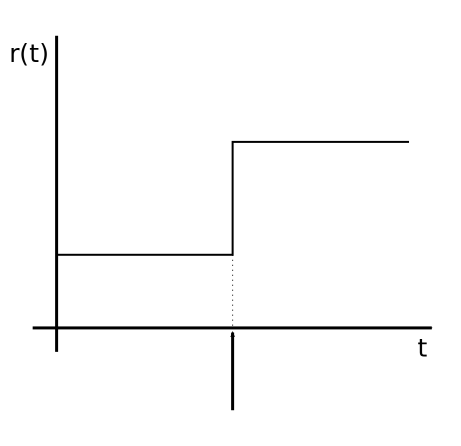
\includegraphics[width=\linewidth]{img/piecewise-setpoint}
			\end{column}
		\end{columns}
		$\Rightarrow$ Add a low-pass filter to the derivative term:
		\begin{equation*}
			\frac{U_d(s)}{E(s)} = \frac{K_d s}{1+s\tau}
		\end{equation*}
		With $s=j\omega$, breakpoint at $\omega=1/\tau$. This prevents amplification of high frequencies. 
\end{frame}

\begin{frame}
	\frametitle{Alternative Derivative Action (Continuous-time)}
	\begin{equation*}
		\frac{U_d(s)}{E(s)} = \frac{K_d s}{1+s\tau}
	\end{equation*}
	
	Further $e(t)$ is replaced by $c\cdot r(t)-y(t)$ with $c$ the setpoint weighting, which is often set to zero to further reduce immediate influence of a sudden set-point jump. \\
	\vspace{1em}
	In the time-domain:
	\begin{equation*}
		u_d(t) = -\tau\frac{du_d}{dt} + K_d \frac{d}{dt}(c\cdot r(t)-y(t))
	\end{equation*}
\end{frame}

\section{Implementations}

\subsection{Analog Implementation}

\begin{frame}
	\frametitle{Analog Implementation}
	The key building block is the operational amplifier (op-amp).
	\begin{columns}
		\begin{column}{0.7 \textwidth}
			\begin{figure}
				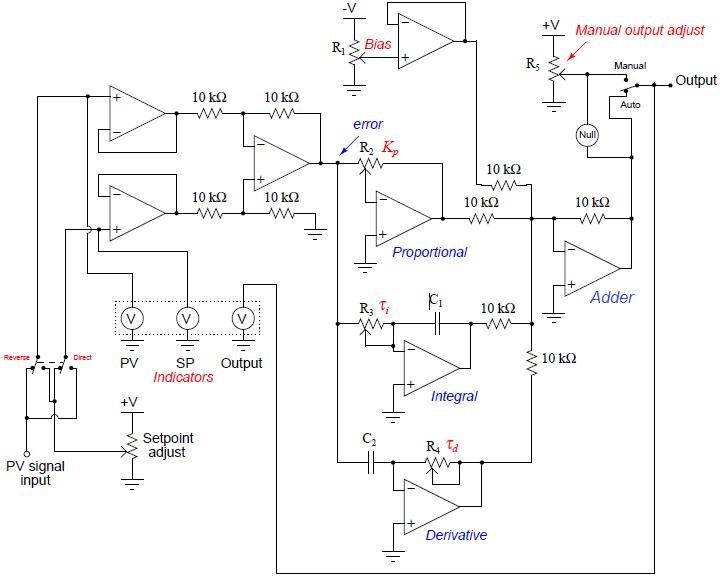
\includegraphics[width=1\linewidth]{analog_example2}
			\end{figure}
		\end{column}
		\begin{column}{0.3 \textwidth}
			\tiny{
				\begin{itemize}
					\item PV - Process Variable $y(t)$
					\item SP - Setpoint $r(t)$
					\item Output - Control action $u(t)$
				\end{itemize}
			}
		\end{column}
	\end{columns}
\end{frame}

\begin{frame}
	\frametitle{Analog Implementation}
	\begin{columns}
		\begin{column}{0.3\linewidth}
			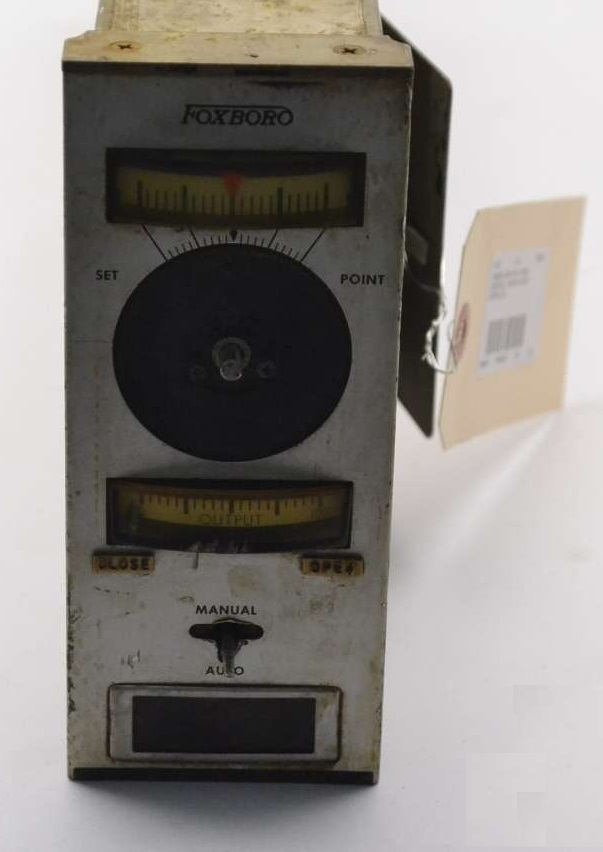
\includegraphics[height=0.6\textheight]{img/FB2a}
		\end{column}
		\begin{column}{0.2\linewidth}
			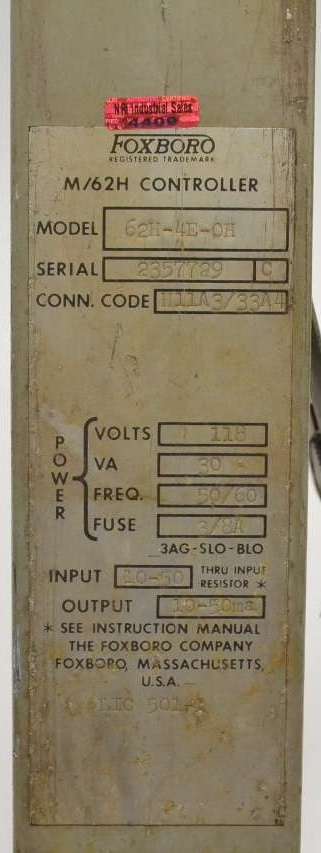
\includegraphics[height=0.6\textheight]{img/fb3a}
		\end{column}
		\begin{column}{0.5\linewidth}
			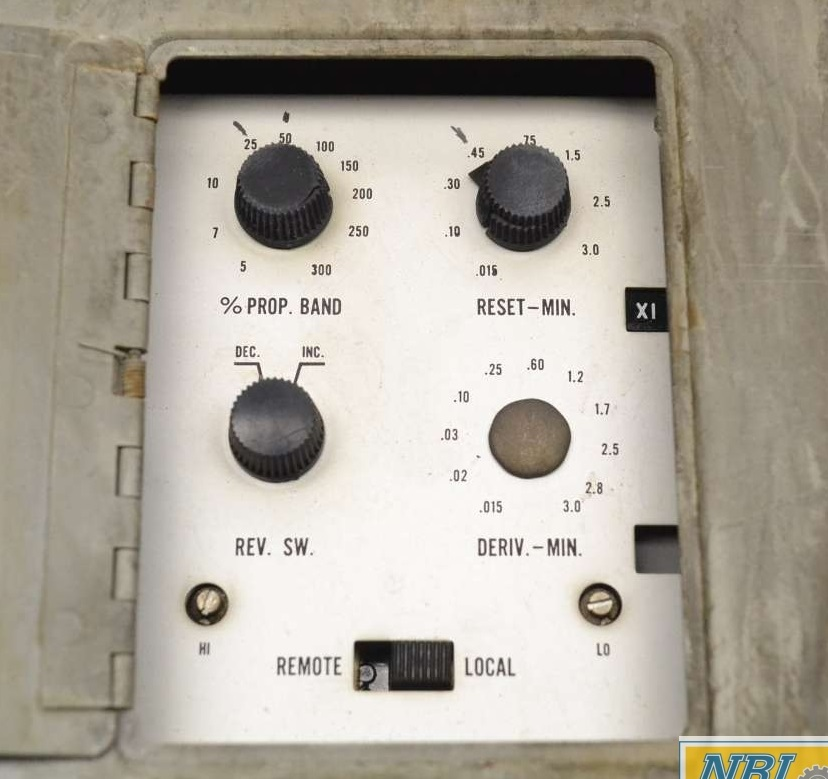
\includegraphics[height=0.6\textheight]{img/fb4}
		\end{column}
	\end{columns}
	\begin{center}
		\textbf{Analog PID controller: FOXBORO 62H-4E-OH M/62H}
	\end{center}
\end{frame}

\begin{frame}{Analog PI Motor Speed Control}
	\begin{figure}
		\centering
		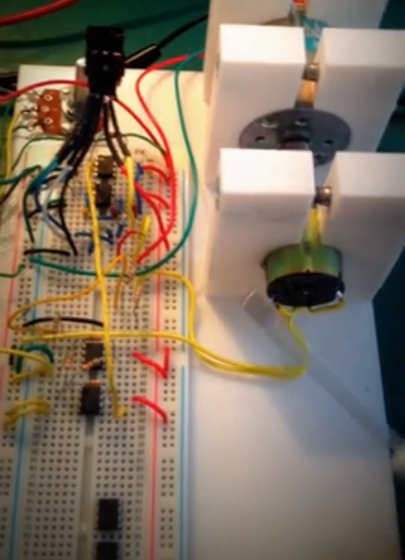
\includegraphics[width=0.4\linewidth]{img/feedback_motor}
	\end{figure}
	\url{https://youtu.be/6W3PLiVIcmE}
\end{frame}

\subsection{Digital Implementation}

\begin{frame}[fragile]
	\frametitle{Digital Implementation}
	\small{
	The difference equations are typically implemented in a microcontroller or in an FPGA  (field-programmable gate array) device:
	\vspace{-0.5em}
		\begin{align*}
		u[k] &= K_p e[k] + \frac{K_d}{T_s}(e[k] - e[k-1])+u_i[k] \\
		&\text{with } u_i[k] = u_i[k-1] + K_i T_s e[k]
		\end{align*}
	}
	\vspace{-1.5em}
	\begin{block}{Pseudocode}
		\hbox{\hspace{0em}
		\begin{lstlisting}[basicstyle=\scriptsize]
			previous_error = 0
			integral = 0
			Start:
			<@\hspace{0.5cm}@> error = setpoint - measured_value
			<@\hspace{0.5cm}@> proportional = KP * error
			<@\hspace{0.5cm}@> integral = integral + Ki*sampling_time*error
			<@\hspace{0.5cm}@> derivative = Kd*(error-previous_error)/sampling_time
			<@\hspace{0.5cm}@> output = proportional + integral + derivative
			<@\hspace{0.5cm}@> previous_error = error
			<@\hspace{0.5cm}@> <@\textcolor{blue}{wait}@> (sampling_time)
			<@\hspace{0.5cm}@> <@\textcolor{blue}{goto}@> Start
		\end{lstlisting}
	}
%	\begin{enumerate}
%		\item Wait for clock interrupt
%		\item Read analog input
%		\item Compute control signal
%		\item Set analog output
%		\item Update controller variables
%		\item Go to 1
%	\end{enumerate}
	\end{block}
\end{frame}

\begin{frame}
	\frametitle{Digital Implementation}
	\begin{columns}
		\begin{column}{0.5\linewidth}
			\centering PLC with a digital PID module:
			
			\vspace{1em}
			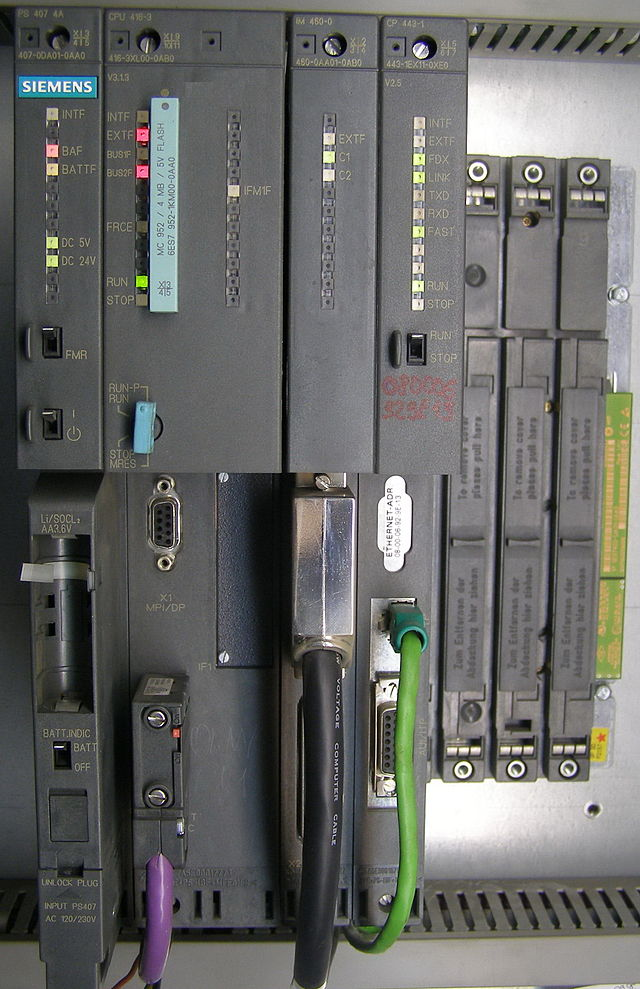
\includegraphics[height=0.7\textheight]{img/640px-Siemens_Simatic_S7-416-3}
		\end{column}
		\begin{column}{0.5\linewidth}
			\centering Digital PID:
			\vspace{1em}
			\begin{columns}
				\begin{column}{0.4\linewidth}
					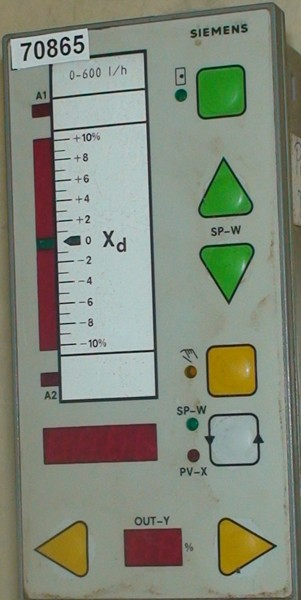
\includegraphics[height=0.7\textheight]{img/278}

				\end{column}
				\begin{column}{0.6\linewidth}
					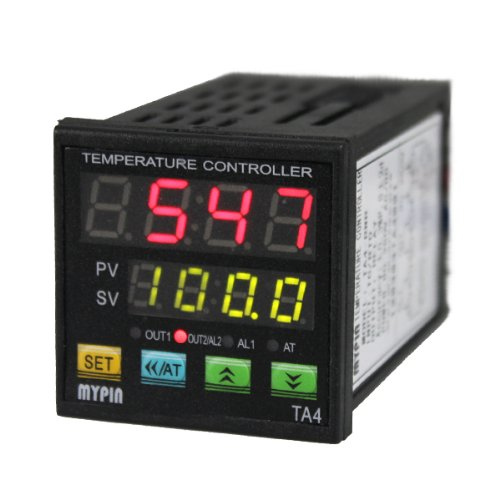
\includegraphics[height=0.4\textheight]{img/41LH64+SGWL}

				\end{column}
			\end{columns}
		\end{column}
	\end{columns}
\end{frame}

\begin{frame}{PLC}
	A \textbf {P}rogrammable \textbf{L}ogic \textbf{C}ontroller (PLC) is a digital computer used for automation in process industry. 
	\begin{columns}
		\begin{column}{0.5\textwidth}
			\begin{figure}
				\centering
				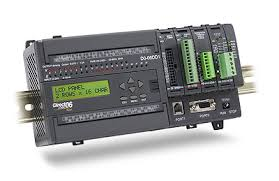
\includegraphics[width=0.7\linewidth]{img/PLC_1}
			\end{figure}

		\end{column}
		\begin{column}{0.5\textwidth}
			\begin{figure}
				\centering
				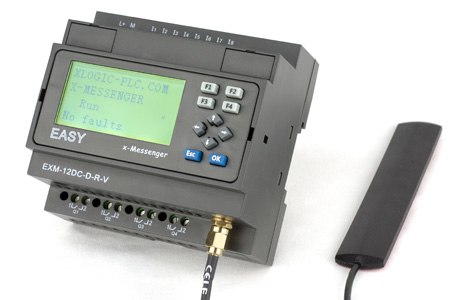
\includegraphics[width=0.7\linewidth]{img/PLC_2}
			\end{figure}
		\end{column}
	\end{columns}
\end{frame}

\begin{frame}{What is a PLC? Basics of PLCs}
	\begin{figure}
		\centering
		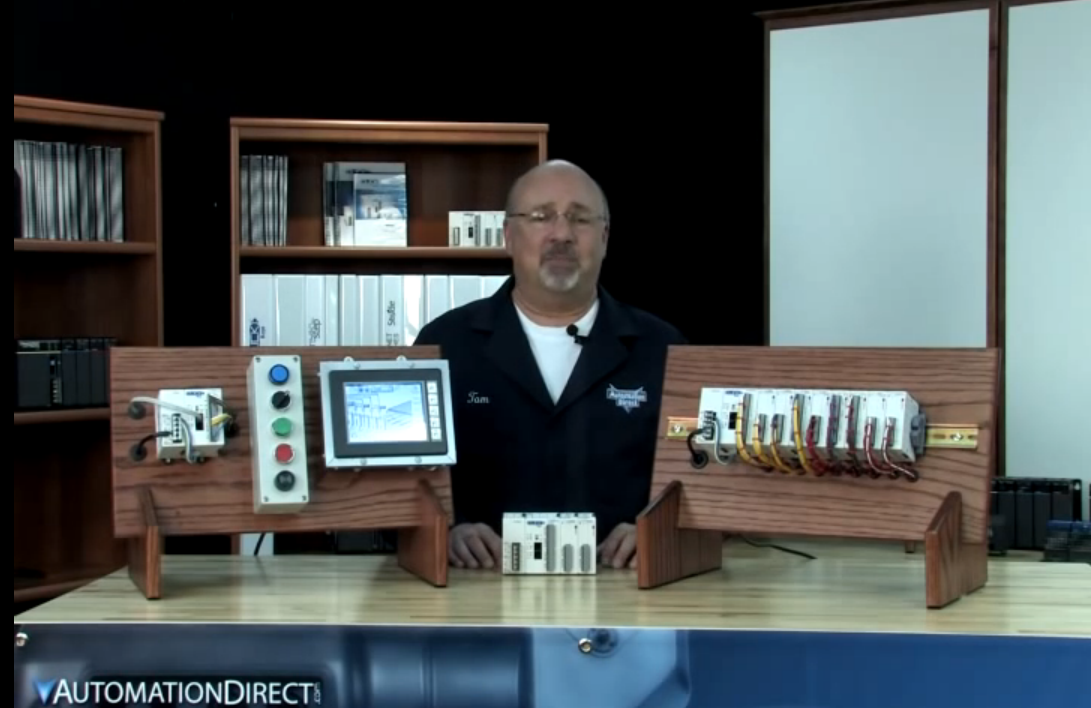
\includegraphics[width=0.7\linewidth]{img/what_is_a_plc}
	\end{figure}
	\url{https://youtu.be/iWgHqqunsyE}
\end{frame}


\section{PID Tuning}

\subsection{Manual Tuning}

\begin{frame}
	\frametitle{Manual Tuning}
	The effects of each of the controller parameters $K_p$, $K_i$,~and~$K_d$ on the closed-loop system are summarized in the table below.
	\vbox{\vspace{1em}
	\hbox{\hspace{-0.6cm}
	{\small
	\begin{tabular}{c | c | c | c | c }
	  \hline
		 \multirow{2}{*}{PID gains}  & \multicolumn{4}{c}{Closed-loop response}\\\cline{2-5}
			&	Rise Time 	&	Overshoot	&	Settling time	&	Steady-State error \\
		\hline
		$K_p \uparrow$ & Decrease	&	Increase	&	Small Change	&	Decrease \\
		$K_i \uparrow$ & Decrease	&	Increase	&	Increase		&	Eliminate \\
		$K_d \uparrow$ & Small change &	Decrease	&	Decrease		&	No change \\
	\end{tabular}
	}
	}
	}
	
	\vspace{1em}
	\begin{alertblock}{Important note}
	Changing one parameter can influence the effect of the other two. Therefore, use this table only as a reference.
	\end{alertblock}
\end{frame}

\begin{frame}
	\frametitle{Manual Tuning}
	One possible way is as follows (the controller is connected to the plant):
	\begin{enumerate}
		\item Set $K_i$ and $K_d$ equal to 0.
		\item Increase $K_p$ until you observe that the step response is fast enough and the steady-state error is small.
		\item Start adding some integral action in order to get rid of the steady-state error. Keep in mind that too much $K_i$ can cause instability!
		\item Add some derivative action in order to quickly react to disturbances and/or dampen the response.
	\end{enumerate}
\end{frame}

\subsection{Heuristic Methods}

\begin{frame}
	\frametitle{Heuristic Methods}
	\justify
	When the \textbf{mathematical model of a plant is unknown} or it is too complicated to obtain, an analytical approach to design a PID controller is not possible. Therefore in these cases we have to use an experimental approach to tune the PID controller.  Among the existing experimental approaches we can mention:
	\begin{itemize}
		\item Ziegler-Nichols tuning rule based on step response (First method)
		\item Ziegler-Nichols tuning rule based on critical gain and critical period (Second method)
	\end{itemize}
\end{frame}

\begin{frame}
	\frametitle{Ziegler-Nichols tuning rule: First Method}
	\justify
	In this method, the response of the plant to a unit-step input is obtained experimentally. If the plant involves neither integrators nor dominant complex-conjugate poles, then such a unit-step response curve may look S-shaped as shown in the figure on the next slide. This S-shaped curve may be characterized by two constants: delay time $L$ and time constant $T$. The delay time and the time constant are determined by drawing a tangent line at the inflection point of the S-shaped curve and determining the intersections of the tangent line with the time axis and a horizontal line crossing the y-axis at point (0,K).
	\begin{alertblock}{}
		If the response to a step input does not exhibit an S-shaped curve, the first method does not apply.
	\end{alertblock}
\end{frame}

\begin{frame}
	\frametitle{Ziegler-Nichols tuning rule: First Method}
	\begin{figure}
		\centering
		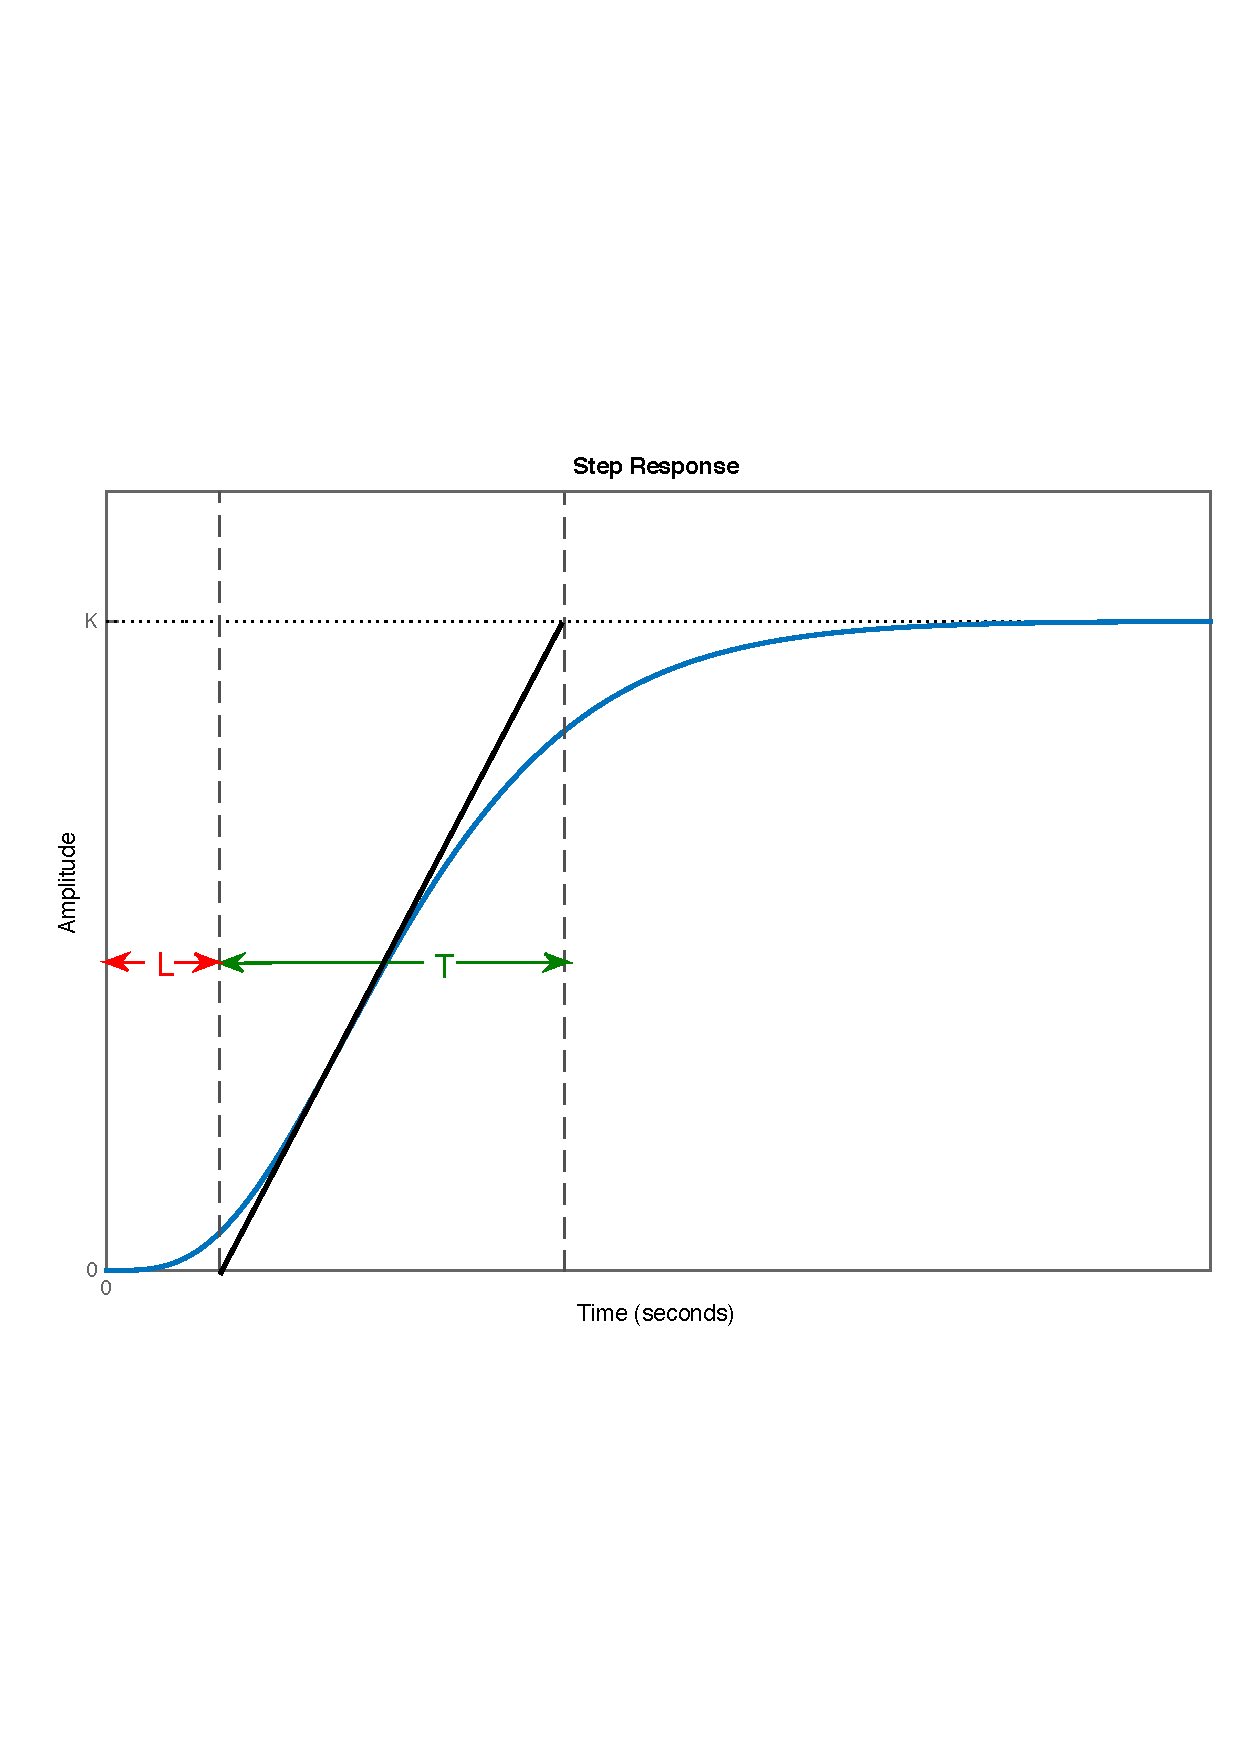
\includegraphics[width=0.8\linewidth]{s_shaped_response}
	\end{figure}
\end{frame}

\begin{frame}
	\frametitle{Ziegler-Nichols tuning rule: First Method}
	Ziegler and Nichols suggested to set the values of $K_p$, $K_i$, and $K_d$  according to the formulas shown in the following table:
	\vbox{\vspace{1em}
		\centering
		\begin{tabular}{c | c | c | c}
		\hline
			Control Type & $K_p$ & $K_i$ & $K_d$\\
			\hline 
			P & $T/L$ & 0 &	0\\[0.5em]
			PI & $0.9\frac{T}{L}$ & $K_p \frac{0.3}{L}$ & 0\\[0.5em]
			PID & $1.2\frac{T}{L}$ & $\frac{K_p}{2L}$ & $0.5 L K_p$ \\
		\end{tabular}}
\end{frame}

\begin{frame}
	\frametitle{Ziegler-Nichols tuning rule: First Method}
	The PID controller tuned by the first method gives:
	\vspace{-0.5em}
	\begin{align*}
		\frac{U(s)}{E(s)} &= K_p + \frac{K_i}{s} + K_d s\\
		&= 1.2\frac{T}{L} \big (1 + \frac{1}{2Ls} + 0.5Ls \big)\\
		&= 0.6 T \frac{\big (s + \frac{1}{L} \big)^2}{s}
	\end{align*}
	with a pole at the origin and a double zero at $s = -\frac{1}{L}$.
\end{frame}

\begin{frame}
	\frametitle{Ziegler-Nichols tuning rule: Second Method}
	This method is based on the value of $K_p$ that results in marginal stability when only proportional control action is used.
	\begin{enumerate}
		\item Set the integral and derivative gains to zero ($K_p$ = $K_d$ = 0);
		\item Increase the proportional gain $K_p$ until the output of the control loop starts oscillating with a constant amplitude. The value of $K_p$ at this point is referred to as ultimate gain ($K_u \triangleq K_p$);
		\item Measure the period of the oscillations $T_u$ at the output of the closed-loop system;
		\item Use $K_u$ and $T_u$ to determine the gains of the PID controller according to the tuning rule table shown in the next slide.
	\end{enumerate}
\end{frame}

\begin{frame}
	\frametitle{Ziegler-Nichols tuning rule: Second Method}
	\vbox{
		\centering
	\begin{tabular}{c | c | c | c}
	 \hline
		Control Type	&	$K_p$		&	$K_i$			&	$K_d$ 	\\
		\hline
		P				&	$0.5K_u$	&	-				&	-		\\
		PI				&	$0.45K_u$	&	$1.2K_p/T_u$		&	-		\\
		PD				&	$0.8K_u$	&	-				&	$K_pT_u/8$ \\
		PID				&	$0.6K_u$	&	$2K_p/T_u$		&	$K_pT_u/8$ \\
		Pessen Integral Rule & $0.7K_u$ &	$2.5K_p/T_u$	&	$3K_pT_u/20$\\
		Some overshoot	&	$0.33K_u$	&	$2K_p/T_u$		&	$K_pT_u/3$	\\
		No overshoot	&	$0.2K_u$	&	$2K_p/T_u$		&	$K_pT_u/3$	\\
	\end{tabular}}
	\begin{alertblock}{}
		If the output does not exhibit sustained oscillations for whatever value $K_p$ may take, then the second method does not apply.
	\end{alertblock}
	\footnotesize{Keep in mind that we are working with heuristic tuning rules, and therefore some additional fine tuning might be necessary.}
\end{frame}

\begin{frame}{Ziegler-Nichols tuning rule: Sedond Method (example)}
	\vspace{-1em}
	\footnotesize{
	\begin{example}
		Consider a plant with a given model:\\
		\vspace{-0.5em}
		$$ P(s) = \frac{1}{(s+1)^3} $$\\
		\vspace{-0.7em}
		\begin{itemize}
		\item We compute the critical gain $K_u$. This is the value of $K_p$ for which $\angle (K_p P(s)) = - 180^\circ$. On the Nyquist plot this is the value of $K_p$ for which $K_p P(s)$ passes through $(-1,0)$.\\
		\end{itemize}
		\vspace{-1.5em}
		\begin{columns}
			\begin{column}{0.5 \textwidth}
				\begin{align*}
				K_uP(j\omega_u) &= -1 \\ \Leftrightarrow K_u &= 	-(j\omega_u + 1)^3 \\
				& = (3\omega_u^2-1)+j(\omega_u^3 - 3\omega_u)
				\end{align*}
				\vspace{-1.5em}
				$$ \omega_u^3-3\omega_u = 0 \Rightarrow \omega_u = \sqrt{3}$$\\
				\vspace{-1.5em}
				$$K_u = 8, T_u = \frac{2\pi}{\omega_u} = 3.628$$\\
				$K_p = 4.8$, $K_i = 2.6448$, $K_d =  2.16$
			\end{column}
			\begin{column}{0.4 \textwidth}
			\begin{figure}
				\centering
				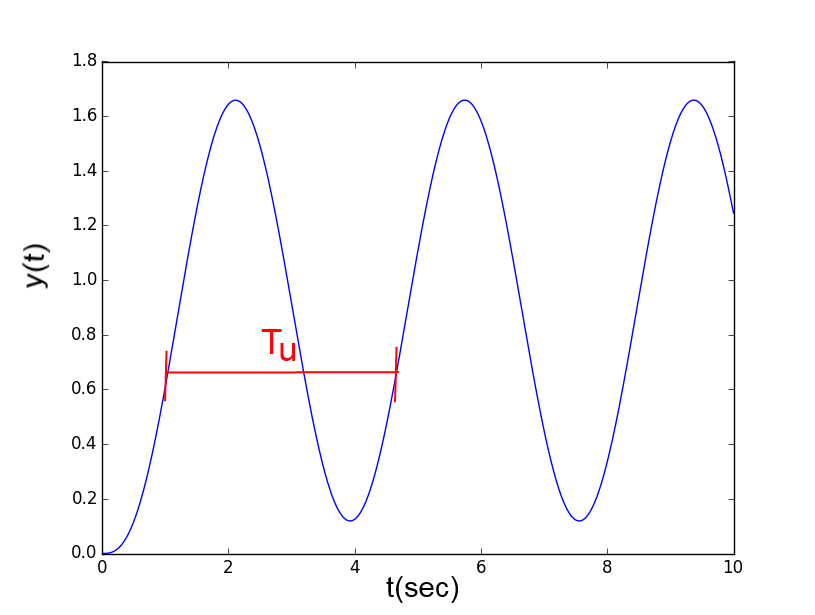
\includegraphics[width=1\linewidth]{img/Z_N_PID_example}
			\end{figure}
			\end{column}
		\end{columns}
	\end{example}}
\end{frame}

\subsection{Numerical Optimization Methods}

\begin{frame}
	\small{
	\frametitle{Numerical Optimization Methods}
	The tuning of a PID controller is posed as a constrained optimization problem.  
	{\footnotesize
	\begin{itemize}
			\item For a given set of parameters $K_p$, $K_i$ and $K_d$ run a simulation of the closed-loop system, and compute some performance parameters (e.g. settling time, rise time, etc.) and a performance index.
			\item Optimize the performance index over the three PID gains.
	\end{itemize}}
	}
	\begin{figure}
	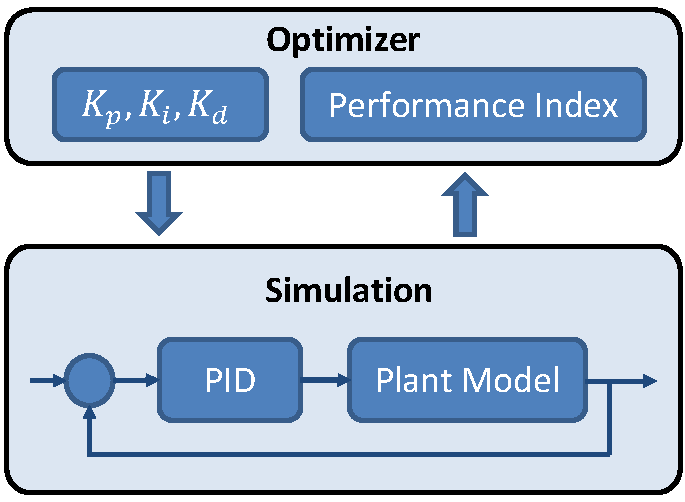
\includegraphics[width=0.5\linewidth]{num_opt}
	\end{figure}	
\end{frame}

\begin{frame}{Some Software Tools}
	\small{
	\begin{tabular}{|p{3cm}|p{7cm}|}
		\hline Software Tool  & Brief Description  \\ 
		\hline pidtool/pidTuner
		 & It is a Matlab tool to interactively design a SISO PID controller in the feed-forward path of single-loop, unity-feedback control configuration \\ 
		\hline Pidpy
		 & It is a modular PID control library for python that supports PID auto tuning. {\color{blue}{\url{https://pypi.python.org/pypi/pypid/}}}
		 \\ 
		\hline INCA PID Tuner
		 & It is a commercial tuning tool developed by IPCOS. It has a vast library of PID structures for DCS and PLC  Systems including Siemens, ABB, Honeywell, Emerson, etc.
		 {\color{blue}{\url{http://www.ipcos.com/advancedprocesscontrol/advanced-process-control/pid-tuning-software/inca-pid-tuning/}}}
		 \\ 
		\hline 
	\end{tabular}}
\end{frame}

\begin{frame}{pidtool/pidTuner - Demo}
	\begin{figure}
		\centering
		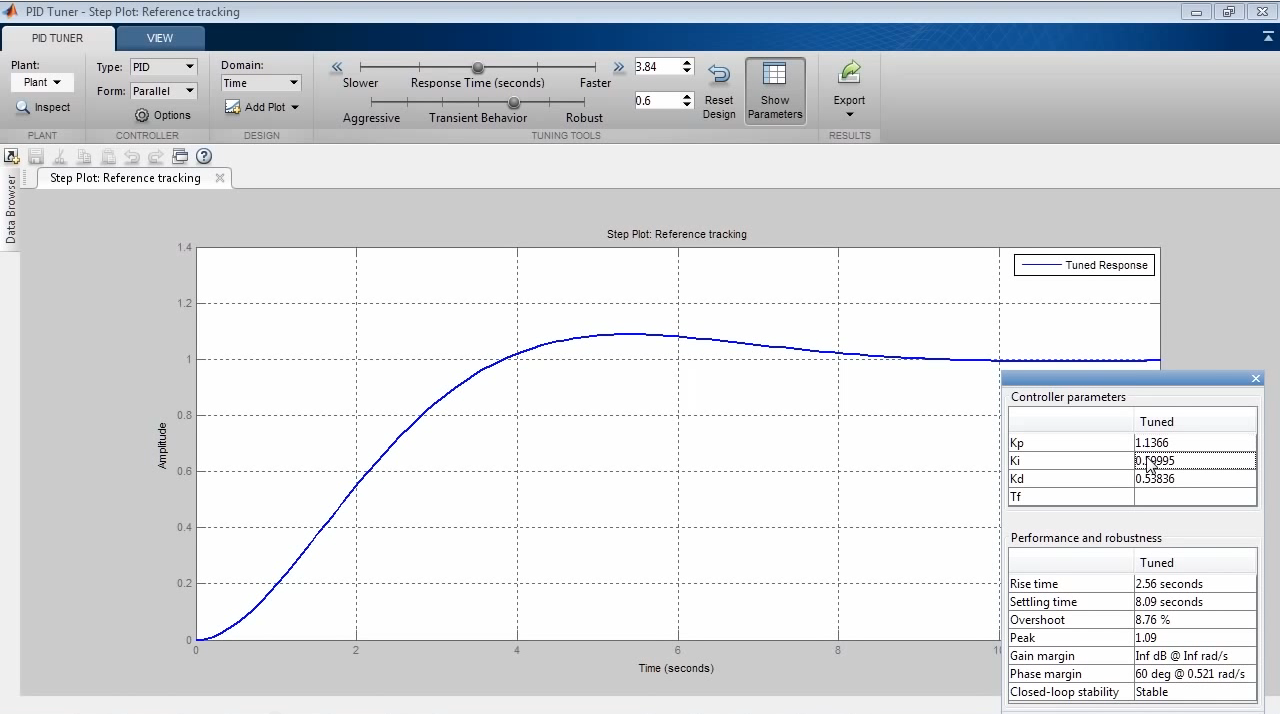
\includegraphics[width=0.7\linewidth]{img/pid_tool}
	\end{figure}
	\url{https://www.youtube.com/watch?v=2tKe0caUv1I}
\end{frame}

\begin{frame}{INCA PID Tuner - Demo}
	\begin{figure}
		\centering
		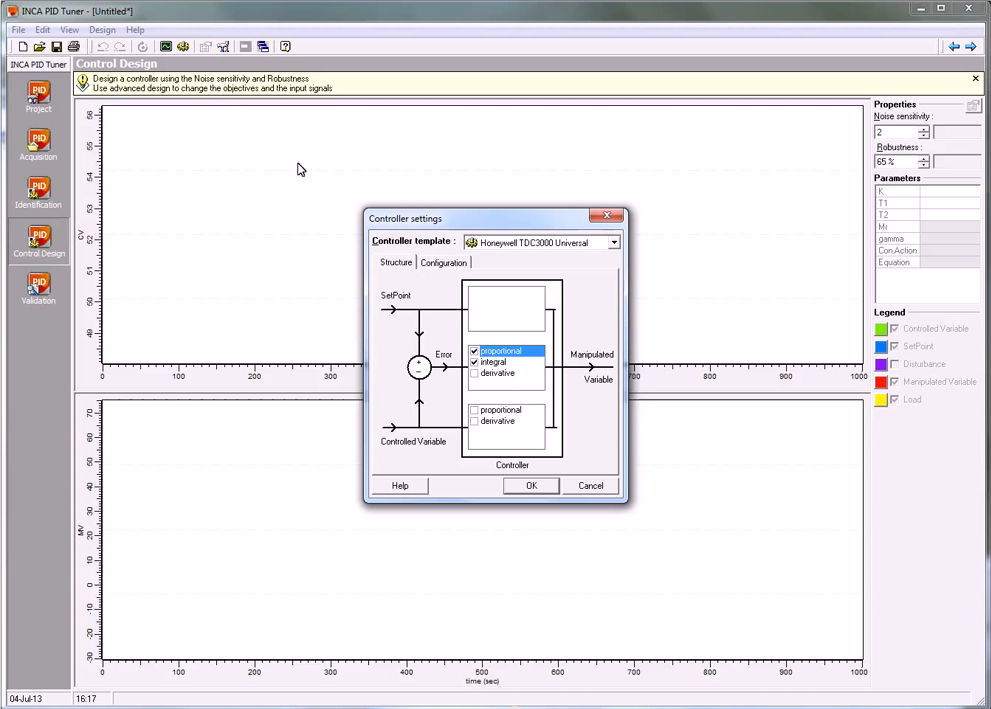
\includegraphics[width=0.7\linewidth]{img/inca_tunner}
	\end{figure}
	\url{https://www.youtube.com/watch?v=XH2bkq1URSg}
\end{frame}